\documentclass{article}
\usepackage[utf8]{inputenc}
\usepackage{graphicx}



\title{zad proj1}
\author{Mateusz Śledzikowski }


\begin{document}

\maketitle

\section{Podpunkt 1}
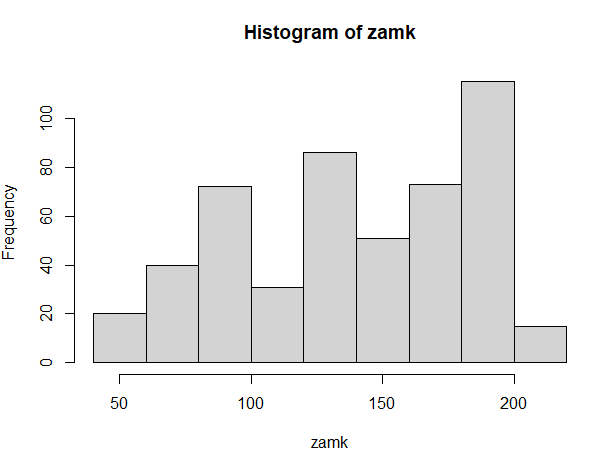
\includegraphics[scale=0.6]{histogram.png}
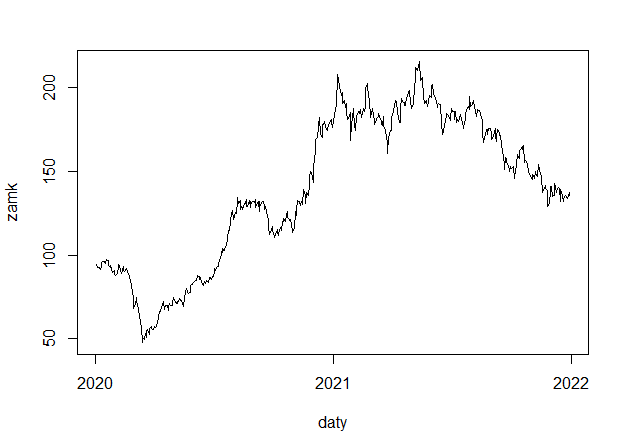
\includegraphics[scale=0.6]{wykres.png}

\section{Podpunkt 2}
Wartość oczekiwana = 139.3693 \\
Odchylenie = 44.12356 \\
\\
Skośność - Miara asymetrii rozkładu. Rozkład normalny jest symetryczny i ma skośność równą 0. Rozkład z dużą skośnością dodatnią ma długi ogon prawostronny. Gdy zaś współczynnik skośności jest ujemny, rozkład ma długi kraniec z lewej strony. Jako wytyczna, wartość skośności przekraczająca dwukrotnie swój błąd standardowy na ogół oznacza odstępstwo od symetrii rozkładu. \\
\\
Kurtoza - Miara zakresu, do którego występują wartości odstające. W przypadku rozkładu normalnego wartość statystyki kurtozy wynosi zero. Kurtoza dodatnia wskazuje, że w danych istnieje więcej dodatnich wartości odstających niż w przypadku rozkładu normalnego. Kurtoza ujemna wskazuje, że w danych istnieje mniej dodatnich wartości odstających niż w przypadku rozkładu normalnego.\\
\\
Skośność = -0.3090048 \\
Kurtoza = -1.164583 \\

\end{document}
